% JUMP TO LINE 60, 75
\documentclass[preview, margin=0.6in]{standalone}
\usepackage[letterpaper,portrait,top=0.4in, left=0.6in, right=0.6in, bottom=1in]{geometry}

\usepackage{amsmath, amsfonts, amsthm, amssymb}
\usepackage{graphicx, float}
\usepackage{mathtools}
\usepackage{titlesec}
\usepackage{interval}
\usepackage{hyperref}
\usepackage{siunitx}
\usepackage{titling}
\usepackage{vwcol}
\usepackage{setspace}
\usepackage{empheq}
\usepackage{cancel}
\usepackage{esdiff}
\usepackage{multicol}
\usepackage{mdframed}
\usepackage{esdiff}
\usepackage{tikzsymbols}
\usepackage{multicol}
\usepackage{tikz}
\usepackage{varwidth}
\usepackage{parskip}
\usepackage{pgfplots}
\usepackage{mlmodern}
\pgfplotsset{compat=1.18}
\intervalconfig {
	soft open fences
}

\newcommand{\alignedintertext}[1]{%
  \noalign{%
    \vtop{\hsize=\linewidth#1\par
    \expandafter}%
    \expandafter\prevdepth\the\prevdepth
  }%
}

\newtheorem{lemma}{Lemma}

\newcommand*{\problem}[1]{\section*{Problem #1}}
\newcommand*{\aps}{\section*{AP Corner}}
\newcommand*{\deriv}[1][x]{\ensuremath{\dfrac{\mathrm{d}}{\mathrm{d}#1}}}
\newcommand*{\floor}[1]{\ensuremath{\lfloor #1\rfloor}}
\newcommand*{\lheqzero}{\ensuremath{\underset{\text{L'H}}{\overset{\left[\frac00\right]}{=}}}}
\newcommand*{\lheqinfty}{\ensuremath{\underset{\text{L'H}}{\overset{\left[\frac{\infty}{\infty}\right]}{=}}}}

\DeclareMathOperator{\DNE}{DNE}
\DeclareMathOperator{\sgn}{sgn}

\DeclareMathOperator{\arccsc}{arccsc}
\DeclareMathOperator{\arcsec}{arcsec}
\DeclareMathOperator{\arccot}{arccot}

%opening

\title{\vspace*{-40pt}Homework Set C.2}
\author{Jayden Li}
\date{\today}
% \allowdisplaybreaks
\postdisplaypenalty=100000

\begin{document}
\setstretch{1.25}
\fontsize{12pt}{12pt}\selectfont
\setlength{\abovedisplayskip}{\abovedisplayskip/2}
\setlength{\belowdisplayskip}{\belowdisplayskip/2}
\setlength{\parindent}{0pt}
\setlength{\parskip}{2ex plus 0.5ex minus 0.2ex}
\maketitle

\problem{2}

Let $u,v,w\in\mathbb R^3$ with components $u=(u_1,u_2,u_3),v=(v_1,v_2,v_3),w=(w_1,w_2,w_3)$.

$\begin{aligned}[t]
	(u+v)\times w
	&=\begin{vmatrix}
		\hat i & \hat j & \hat k \\
		u_1+v_1 & u_2+v_2 & u_3+v_3 \\
		w_1 & w_2 & w_3
	\end{vmatrix}
	=\left\{
	\begin{aligned}
		&\hat i \left( \left( u_2+v_2 \right)w_3-\left( u_3+v_3 \right)w_2 \right)- \\
		&\hat j \left( \left( u_1+v_1 \right)w_3-\left( u_3+v_3 \right)w_1 \right)+ \\
		&\hat k \left( \left( u_1+v_1 \right)w_2-\left( u_2+v_2 \right)w_1 \right)
	\end{aligned}
	\right. \\
	&=\left\{\begin{aligned}
		&\hat i \left( u_2w_3+v_2w_3-u_3w_2-v_3w_2 \right)-\\ 
		&\hat j \left( u_1w_3+v_1w_3-u_3w_1-v_3w_1 \right)+\\ 
		&\hat k \left( u_1w_2+v_1w_2-u_2w_1-v_2w_1 \right)
	\end{aligned}\right. \\
	u\times w+v\times w
	&=
	\begin{vmatrix}
		\hat i & \hat j & \hat k \\
		u_1 & u_2 & u_3 \\
		w_1 & w_2 & w_3 \\
	\end{vmatrix}
	+\begin{vmatrix}
		\hat i & \hat j & \hat k \\
		v_1 & v_2 & v_3 \\
		w_1 & w_2 & w_3 \\
	\end{vmatrix}
	=\left\{ 
		\begin{aligned}
			&\hat i \left( u_2w_3-u_3w_2 \right)- \\
			&\hat j \left( u_1w_3-u_3w_1 \right)+ \\
			&\hat k \left( u_1w_2-u_2w_1 \right)
		\end{aligned}
	\right\}
	+\left\{ 
		\begin{aligned}
			&\hat i \left( v_2w_3-v_3w_2 \right)- \\
			&\hat j \left( v_1w_3-v_3w_1 \right)+ \\
			&\hat k \left( v_1w_2-v_2w_1 \right)
		\end{aligned}
	\right\} \\
	&=\left\{\begin{aligned}
		&\hat i \left( u_2w_3+v_2w_3-u_3w_2-v_3w_2 \right)-\\ 
		&\hat j \left( u_1w_3+v_1w_3-u_3w_1-v_3w_1 \right)+\\ 
		&\hat k \left( u_1w_2+v_1w_2-u_2w_1-v_2w_1 \right)
	\end{aligned}\right\}
	=(u+v)w
\end{aligned}$

\problem{3}
Let $a,b\in\mathbb R^3$. Notice that $a\times(-b)=(-a)\times b=-(a\times b)$.

$\begin{aligned}[t]
	(a-b)\times(a+b)
	&=(a+(-b))\times(a+b)
	=a\times (a+b)+(-b)\times (a+b) \\
	&=a\times a+a\times b+(-b)\times a+(-b)\times b
	=0+a\times b-(b\times a)-(b\times b) \\
	&=0+a\times b-(-(a\times b))-0
	=a\times b +a\times b
	=\boxed{2(a\times b)}
\end{aligned}$

\problem{4}
Let $\theta$ be the angle between the vectors $a$ and $b$.
\begin{center}
	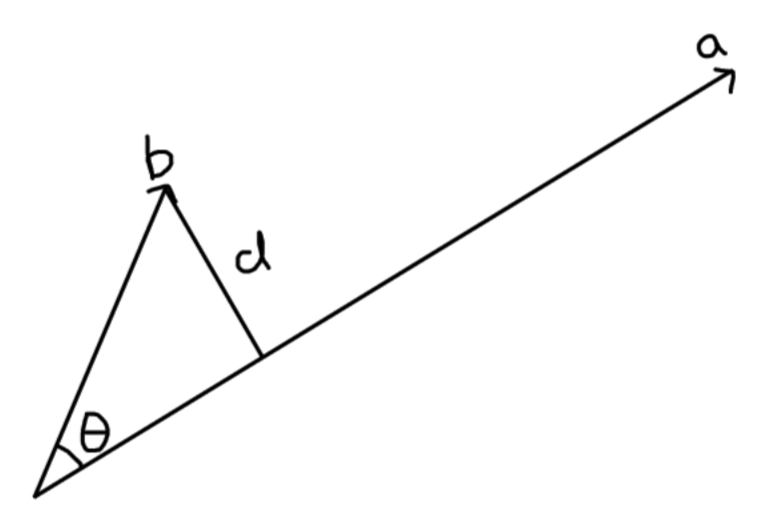
\includegraphics[width=0.4\linewidth]{q4.png}
\end{center}
\begin{equation*}
    \sin\theta=\frac{d}{\lVert b \rVert }
	\implies d
	=\lVert b \rVert \sin\theta
	=\frac{\lVert a \rVert \lVert b \rVert \sin\theta}{\lVert a \rVert }
	=\boxed{\frac{\lVert a\times b \rVert }{\lVert a \rVert }}
\end{equation*}


\end{document}
